\documentclass{article}\usepackage[]{graphicx}\usepackage[]{color}
%% maxwidth is the original width if it is less than linewidth
%% otherwise use linewidth (to make sure the graphics do not exceed the margin)
\makeatletter
\def\maxwidth{ %
  \ifdim\Gin@nat@width>\linewidth
    \linewidth
  \else
    \Gin@nat@width
  \fi
}
\makeatother

\definecolor{fgcolor}{rgb}{0.345, 0.345, 0.345}
\newcommand{\hlnum}[1]{\textcolor[rgb]{0.686,0.059,0.569}{#1}}%
\newcommand{\hlstr}[1]{\textcolor[rgb]{0.192,0.494,0.8}{#1}}%
\newcommand{\hlcom}[1]{\textcolor[rgb]{0.678,0.584,0.686}{\textit{#1}}}%
\newcommand{\hlopt}[1]{\textcolor[rgb]{0,0,0}{#1}}%
\newcommand{\hlstd}[1]{\textcolor[rgb]{0.345,0.345,0.345}{#1}}%
\newcommand{\hlkwa}[1]{\textcolor[rgb]{0.161,0.373,0.58}{\textbf{#1}}}%
\newcommand{\hlkwb}[1]{\textcolor[rgb]{0.69,0.353,0.396}{#1}}%
\newcommand{\hlkwc}[1]{\textcolor[rgb]{0.333,0.667,0.333}{#1}}%
\newcommand{\hlkwd}[1]{\textcolor[rgb]{0.737,0.353,0.396}{\textbf{#1}}}%
\let\hlipl\hlkwb

\usepackage{framed}
\makeatletter
\newenvironment{kframe}{%
 \def\at@end@of@kframe{}%
 \ifinner\ifhmode%
  \def\at@end@of@kframe{\end{minipage}}%
  \begin{minipage}{\columnwidth}%
 \fi\fi%
 \def\FrameCommand##1{\hskip\@totalleftmargin \hskip-\fboxsep
 \colorbox{shadecolor}{##1}\hskip-\fboxsep
     % There is no \\@totalrightmargin, so:
     \hskip-\linewidth \hskip-\@totalleftmargin \hskip\columnwidth}%
 \MakeFramed {\advance\hsize-\width
   \@totalleftmargin\z@ \linewidth\hsize
   \@setminipage}}%
 {\par\unskip\endMakeFramed%
 \at@end@of@kframe}
\makeatother

\definecolor{shadecolor}{rgb}{.97, .97, .97}
\definecolor{messagecolor}{rgb}{0, 0, 0}
\definecolor{warningcolor}{rgb}{1, 0, 1}
\definecolor{errorcolor}{rgb}{1, 0, 0}
\newenvironment{knitrout}{}{} % an empty environment to be redefined in TeX

\usepackage{alltt}
\IfFileExists{upquote.sty}{\usepackage{upquote}}{}
\begin{document}
\begin{figure}
\begin{knitrout}
\definecolor{shadecolor}{rgb}{0.969, 0.969, 0.969}\color{fgcolor}\begin{kframe}
\begin{alltt}
\hlkwd{layout}\hlstd{(}\hlkwd{matrix}\hlstd{(}\hlkwd{c}\hlstd{(}\hlnum{1}\hlstd{,}\hlnum{3}\hlstd{,}\hlnum{0}\hlstd{,}\hlnum{0}\hlstd{,}\hlnum{2}\hlstd{,}\hlnum{4}\hlstd{),} \hlnum{2}\hlstd{,} \hlnum{3}\hlstd{),} \hlkwc{respect} \hlstd{=} \hlnum{TRUE}\hlstd{,}
\hlkwc{widths}\hlstd{=}\hlkwd{c}\hlstd{(}\hlnum{7.5}\hlstd{,}\hlnum{1}\hlstd{,}\hlnum{7.5}\hlstd{),} \hlkwc{heights}\hlstd{=}\hlkwd{c}\hlstd{(}\hlnum{7.5}\hlstd{,} \hlnum{1.5}\hlstd{))}
\hlstd{xlim} \hlkwb{<-} \hlkwd{range}\hlstd{(DAAG}\hlopt{::}\hlstd{nihills}\hlopt{$}\hlstd{time)}\hlopt{+}\hlkwd{c}\hlstd{(}\hlopt{-}\hlnum{0.1}\hlstd{,}\hlnum{0.1}\hlstd{)}
\hlkwd{par}\hlstd{(}\hlkwc{mar}\hlstd{=}\hlkwd{c}\hlstd{(}\hlnum{0.2}\hlstd{,}\hlnum{2.5}\hlstd{,}\hlnum{0}\hlstd{,}\hlnum{0}\hlstd{),} \hlkwc{bty}\hlstd{=}\hlstr{"o"}\hlstd{)}
\hlkwd{plot}\hlstd{(timef}\hlopt{~}\hlstd{time,} \hlkwc{data}\hlstd{=DAAG}\hlopt{::}\hlstd{nihills,} \hlkwc{xlim}\hlstd{=xlim,} \hlkwc{xaxt}\hlstd{=}\hlstr{'n'}\hlstd{,} \hlkwc{fg}\hlstd{=}\hlstr{"gray"}\hlstd{)}
\hlkwd{mtext}\hlstd{(}\hlkwc{side}\hlstd{=}\hlnum{2}\hlstd{,}\hlkwc{line}\hlstd{=}\hlnum{2}\hlstd{,}\hlstr{"Female times"}\hlstd{)}
\hlkwd{mtext}\hlstd{(}\hlkwc{side}\hlstd{=}\hlnum{3}\hlstd{,}\hlkwc{line}\hlstd{=}\hlnum{0.5}\hlstd{,}\hlstr{"A: Untransformed scales"}\hlstd{,} \hlkwc{adj}\hlstd{=}\hlnum{0}\hlstd{)}
\hlkwd{plot}\hlstd{(timef}\hlopt{~}\hlstd{time,} \hlkwc{data}\hlstd{=DAAG}\hlopt{::}\hlstd{nihills,} \hlkwc{xlim}\hlstd{=xlim,} \hlkwc{xaxt}\hlstd{=}\hlstr{'n'}\hlstd{,}
     \hlkwc{log}\hlstd{=}\hlstr{'xy'}\hlstd{,} \hlkwc{fg}\hlstd{=}\hlstr{"gray"}\hlstd{)}
\hlkwd{mtext}\hlstd{(}\hlkwc{side}\hlstd{=}\hlnum{2}\hlstd{,}\hlkwc{line}\hlstd{=}\hlnum{2}\hlstd{,}\hlstr{"Female times (log scale)"}\hlstd{)}
\hlkwd{mtext}\hlstd{(}\hlkwc{side}\hlstd{=}\hlnum{3}\hlstd{,}\hlkwc{line}\hlstd{=}\hlnum{0.5}\hlstd{,}\hlstr{"B: Logarithmic scales"}\hlstd{,} \hlkwc{adj}\hlstd{=}\hlnum{0}\hlstd{)}
\hlkwd{par}\hlstd{(}\hlkwc{mar}\hlstd{=}\hlkwd{c}\hlstd{(}\hlnum{2}\hlstd{,}\hlnum{2.5}\hlstd{,}\hlnum{0}\hlstd{,}\hlnum{0}\hlstd{),} \hlkwc{bty}\hlstd{=}\hlstr{"n"}\hlstd{)}
\hlstd{pars} \hlkwb{=} \hlkwd{list}\hlstd{(}\hlkwc{boxwex} \hlstd{=} \hlnum{4.0}\hlstd{,} \hlkwc{staplewex} \hlstd{=} \hlnum{0.5}\hlstd{,} \hlkwc{outwex} \hlstd{=} \hlnum{0.5}\hlstd{)}
\hlkwd{boxplot}\hlstd{(DAAG}\hlopt{::}\hlstd{nihills}\hlopt{$}\hlstd{time,} \hlkwc{horizontal}\hlstd{=T,} \hlkwc{xlim}\hlstd{=xlim,}
        \hlkwc{pars}\hlstd{=pars,} \hlkwc{at}\hlstd{=}\hlnum{2}\hlstd{,} \hlkwc{axes}\hlstd{=}\hlnum{0}\hlstd{)}
\hlkwd{axis}\hlstd{(}\hlnum{1}\hlstd{,} \hlkwc{lwd} \hlstd{=} \hlnum{0}\hlstd{,} \hlkwc{lwd.ticks} \hlstd{=} \hlnum{1}\hlstd{)}
\hlkwd{mtext}\hlstd{(}\hlkwc{side}\hlstd{=}\hlnum{1}\hlstd{,}\hlkwc{line}\hlstd{=}\hlnum{2}\hlstd{,}\hlstr{"Male times"}\hlstd{)}
\hlkwd{boxplot}\hlstd{(DAAG}\hlopt{::}\hlstd{nihills}\hlopt{$}\hlstd{time,} \hlkwc{horizontal}\hlstd{=T,} \hlkwc{xlim}\hlstd{=xlim,}
        \hlkwc{log}\hlstd{=}\hlstr{'x'}\hlstd{,} \hlkwc{pars}\hlstd{=pars,} \hlkwc{at}\hlstd{=}\hlnum{2}\hlstd{,} \hlkwc{axes}\hlstd{=}\hlnum{0}\hlstd{)}
\hlkwd{axis}\hlstd{(}\hlnum{1}\hlstd{,} \hlkwc{lwd} \hlstd{=} \hlnum{0}\hlstd{,} \hlkwc{lwd.ticks} \hlstd{=} \hlnum{1}\hlstd{)}
\hlkwd{mtext}\hlstd{(}\hlkwc{side}\hlstd{=}\hlnum{1}\hlstd{,}\hlkwc{line}\hlstd{=}\hlnum{2}\hlstd{,}\hlstr{"Male times (log scale)"}\hlstd{)}
\end{alltt}
\end{kframe}
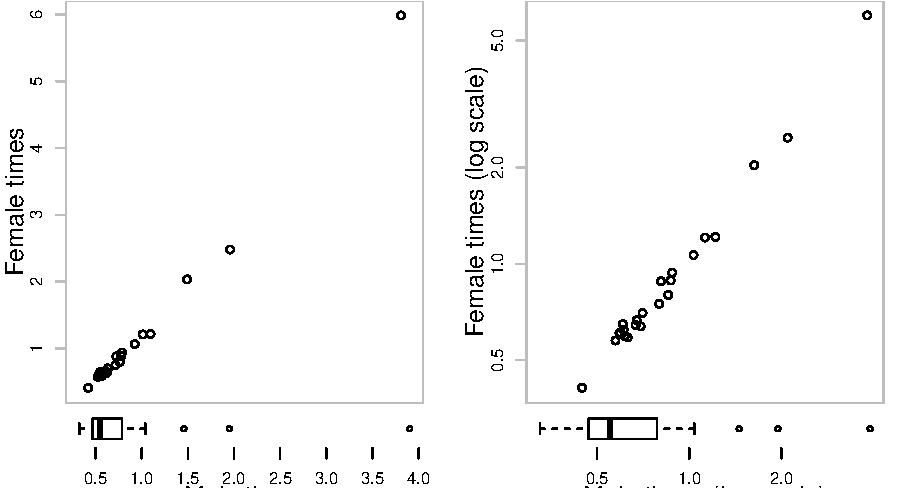
\includegraphics[width=\maxwidth]{figure/A-1} 

\end{knitrout}
\end{figure}
\end{document}
